\chapter{Managing SSH}

\section{Understanding Secure SSH Authentication}
Using ssh we can start a shell session on another server. As such, the usual method of authenticating with passwords is still applicable, but in addition, encryption keys can be used. The primary advantage is that while passwords can be guessed, keys can't!

We generate the SSH keys using a command called \verb|ssh-keygen| which produces two files, i.e., a key-pair, named (by default): the private key \verb|~/.ssh/id_rsa| and the public key \verb|~/.ssh/id_rsa.pub|. This public key has to be copied over to the server so that it can verify that it's really us that's connecting. For this we can use a command \verb|ssh-copy-id|. This command copies the contents of our public key to a file on the server (for the same user) called \verb|~/.ssh/authorized_keys|. 

Now when we authenticate to initiate the ssh session, an authentication token will be generated, which will be encrypted with our private key (on the client). The private key itself is never transported over the network! The encrypted token instead is sent to the server, where it is decrypted using our public key stored in the \verb|authorized_keys| file. The validity of the token determines our authentication (since a file encrypted with our \textit{private key} can only be decrypted with our \textit{public key}, thus confirming our identity to the server).

In case the private key is stolen however, anyone with it can login to the server pretending to be us, and thus it's best practice to encrypt the private key itself with a \textit{passphrase}, which is like a password that allows us to use the private key. This means that the passphrase still has to be typed every time we want to connect via SSH (unless the passphrase is stored in the \textit{keyring}), but this is an extremely secure means of communication due to the nature of public key cryptography and the fact that no passwords (or passphrases) are ever transported over the network!

\section{Configuring Key-based Authentication}
Normally, logging into another server would involve:

\vspace{-15pt}
\begin{minted}{console}
# ssh deux.vm.somuvmnet.local
The authenticity of host 'deux.vm.somuvmnet.local (10.0.99.12)' can't be established.
ECDSA key fingerprint is SHA256:FXXYSAjWZKQHVQpk0EQExJHGgWogmI6GX5nvEvAnIkw.
ECDSA key fingerprint is MD5:0a:8d:8a:69:15:f0:ef:a2:0e:eb:c6:4b:6b:00:70:33.
Are you sure you want to continue connecting (yes/no)? yes
Warning: Permanently added 'deux.vm.somuvmnet.local' (ECDSA) to the list of known hosts.
root@deux.vm.somuvmnet.local's password: 
Last login: Fri Mar 23 23:35:49 2018
#
\end{minted}
\vspace{-10pt}	

\noindent
However, if we're to use a SSH key to login. For this, we can specify tat we want DSA algorithm for the key pair, since it's a bit more secure than the default RSA option. We can create the key and then install it on the target server with:

\vspace{-15pt}
\begin{minted}{console}
# ssh-keygen -t dsa
Generating public/private dsa key pair.
Enter file in which to save the key (/root/.ssh/id_dsa): 
Enter passphrase (empty for no passphrase): 
Enter same passphrase again: 
Your identification has been saved in /root/.ssh/id_dsa.
Your public key has been saved in /root/.ssh/id_dsa.pub.
The key fingerprint is:
SHA256:l6qZh8C0XlrfiaTIJaVVRMjOwjCT/Yi3s8fg1YxMGxs root@prime.vm.somuvmnet.local
The key's randomart image is:
+---[DSA 1024]----+
|   o . +o        |
|  = . o .        |
|   * = .         |
|  . * E    .     |
|   + X OS o      |
|    X X +o       |
|   + # =.o .     |
|    B =++ o      |
|     .+.         |
+----[SHA256]-----+
# ssh-copy-id deux.vm.somuvmnet.local
/usr/bin/ssh-copy-id: INFO: Source of key(s) to be installed: "/root/.ssh/id_dsa.pub"
/usr/bin/ssh-copy-id: INFO: attempting to log in with the new key(s), to filter out any that are already installed
/usr/bin/ssh-copy-id: INFO: 1 key(s) remain to be installed -- if you are prompted now it is to install the new keys
root@deux.vm.somuvmnet.local's password: 

Number of key(s) added: 1

Now try logging into the machine, with:   "ssh 'deux.vm.somuvmnet.local'"
and check to make sure that only the key(s) you wanted were added.

# ssh deux.vm.somuvmnet.local
Enter passphrase for key '/root/.ssh/id_dsa': 
Last login: Fri Mar 23 23:38:34 2018 from deux.vm.somuvmnet.local
# hostname
deux.vm.somuvmnet.local
# cat .ssh/authorized_keys
ssh-dss AAAA ... b0VQ== root@prime.vm.somuvmnet.local
\end{minted}
\vspace{-10pt}	

\noindent
Thus, the ssh-copy-id command merely copies the contents of the public key from the \verb|id_dsa.pub| file on the client to the \verb|authorized_keys| of the host we're trying to connect to. 

\subsection{Removing the need to re-enter passphrase}
To remove the need to continually re-enter the SSH passphrase, we can simply start a new sub-shell under the ssh-agent and then add the identity of the user by linking the passphrase for the current user with the sub-shell, using ssh-add. The procedure is:

\vspace{-15pt}
\begin{minted}{console}
# ssh-agent /bin/bash
# ssh-add
Enter passphrase for /root/.ssh/id_dsa: 
Identity added: /root/.ssh/id_dsa (/root/.ssh/id_dsa)
# ssh deux.vm.somuvmnet.local 
Last login: Fri Mar 23 23:43:07 2018 from prime.vm.somuvmnet.local
# exit
logout
Connection to deux.vm.somuvmnet.local closed.
# ssh deux.vm.somuvmnet.local 
Last login: Fri Mar 23 23:49:39 2018 from prime.vm.somuvmnet.local
# exit
logout
Connection to deux.vm.somuvmnet.local closed.
# exit
exit
# # Exited the ssh-agent sub-shell
# ssh deux.vm.somuvmnet.local 
Enter passphrase for key '/root/.ssh/id_dsa': 
Last login: Fri Mar 23 23:49:45 2018 from prime.vm.somuvmnet.local
\end{minted}
\vspace{-10pt}	

\noindent
The \verb|ssh-add| command is used to add the contents of the private key to the authentication agent on the local machine. We \textit{have} to use this command in a sub-shell because we don't want the credentials to be attached to the authentication agent of our own (parent) terminal session, but the child-shell created by the \verb|ssh-agent| command. Note however, that the authentication is valid \textit{only} till the shell that it's attached to (in our case, the child shell started with \verb|ssh-agent|).

If we'd choose to use \verb|ssh-agent|, it's a great option, but typically requires the passphrase be re-entered after logging in to ensure that the key is cached. 

\subsection{Turning off password-based authentication} 
The \verb|/etc/ssh/sshd_config| file controls the configuration of the SSH daemon and it can be configured to only allow authentication via key-based authentication for SSH sessions. This'd mean that anybody who already doesn't have a key that's present in the \verb|authorized_hosts| file on the server can't login to it. We can do this by changing the value of \verb|PasswordAuthentication| to \textbf{no}:

\vspace{-15pt}
\begin{minted}{bash}
PasswordAuthentication no
\end{minted}
\vspace{-10pt}	

\noindent
Note that simply commenting out the line won't work, and the value has to be explicitly changed to \textbf{no}. Then we have to use \verb|systemctl restart sshd| to restart the \textbf{sshd} service for the changes to take effect. Then, when someone without a key tries to log in to the server, the get a \textit{Permisson denied} error, stating:

\vspace{-15pt}
\begin{minted}{console}
# ssh prime.vm.somuvmnet.local
Permission denied (publickey,gssapi-keyex,gssapi-with-mic).
\end{minted}
\vspace{-10pt}	

\noindent
While this method is very secure, this isn't very convenient and thus many admins decide to leave it on. 

	\section{Understanding Important SSH Options}
Some of the useful options in the \verb|/etc/ssh/sshd_config| file to customize SSH operation are:

\noindent
\begin{tabular}{rM{0.45}M{0.27}}
	\toprule
	\textbf{Terms} &\textbf{Description} &\textbf{Default Val}\\
	\midrule
	\textbf{Port}	&The port on which incoming connections for SSH will be allowed. Default value is fine, unless server accepts SSH through internet, in which cases port 22 invites trouble. &\verb|Port 22|\\
	\midrule
	\textbf{ListenAddress}	&The IP address on which incoming SSH connections will be anticipated. Controls which interface the incoming SSH connections should use. &\verb|ListenAddress 0.0.0.0|\\
	\midrule
	\textbf{SyslogFacility}	&Determines which facility (and consequently which log) is used by syslog to log the events of SSH. The LogLevel sets the urgency in logs. &\verb|SyslogFacility AUTHPRIV| \verb|LogLevel INFO|\\
	\midrule
	\textbf{PermitRootLogin}	&By default the users who use SSH can login as root as well, but if this is set to no, the root user can only login via other means and not through SSH. Useful for login purposes. &\verb|PermitRootLogin yes|\\
	\midrule
	\textbf{AllowUsers}	&Allows only specific users to login via SSH. Any user not on this list will be denied entry. . From this point onwards, only the users mentioned are allowed to login, even when \verb|PermitRootLogin| is set to yes. &None; Syntax: \verb|AllowUsers <username>| \\
	\midrule
	\textbf{MaxSessions} &Useful in situations where high SSH traffic is expected and thus many concurrent SSH sessions may have to run. &\verb|MaxSessions 10|\\
	\midrule
	\textbf{GSSAPI*} &A bunch of API options for Centralized Directory Server authentication like Kerberos and Active Directory. This being switched off makes the authentication process a bit faster. thus, these should only be used when required. &\verb|GSSAPIAuthentication yes| \verb|GSSAPICleanupCredentials no| \verb|GSSAPIStrictAcceptorCheck yes| \verb|GSSAPIKeyExchange no| \verb|GSSAPIEnablek5users no|		\\
	\midrule
	\textbf{X11Forwarding} &\textbf{X11} is a communication protocol that enables GUI transmission. In case of X11 forwarding, the user is presented with a single window of application that he can view on their monitor via SSH. Unlike VNC, a session isn't established and only a single window is sent to the client. &\verb|X11Forwarding yes|\\
	\midrule
	\textbf{TCPKeepAlive} &Ensure that a SSH connection isn't broken or terminated after a period of inactivity. Can be used in conjunction with \textit{ClientAliveInterval} and \textit{ClientAliveCountMax}. &\verb|TCPKeepAlive yes|\\
	\bottomrule		
\end{tabular}

\noindent
\begin{tabular}{rM{0.45}M{0.27}}
	\toprule
	\textbf{Terms} &\textbf{Description} &\textbf{Default Val}\\
	\midrule
	\textbf{ClientAliveInterval} &ClientAliveInterval is used by the server to check if the client is still alive after a period of inactivity. This is useful because it helps keep SSH session open. The default value of 0 means that the messages won't be sent to the client (via a secure channel) to check their state. These messages unlike TCPKeepAlive are non-spoofable and encrypted. &\verb|ClientAliveInterval 0|\\
	\midrule
	\textbf{ClientAliveCountMax} &Determines the maximum number of messages that'll be sent to the client to ensure it's activity (i.e., connection is still active) without reply from the client before the connection is considered dead and closed. &\verb|ClientAliveCountMax 3|\\
	\bottomrule
\end{tabular}

\subsection{Chaning the SSH Port}
To change the SSH port, simply changing the value of the port parameter in \verb|sshd_config| isn't enough since the SELinux security context of the port won't match. This can be verified by restarting \textbf{sshd} and checking the status after changing the port value:

\vspace{-15pt}
\begin{minted}{console}
# systemctl restart sshd; systemctl status sshd
Job for sshd.service failed because the control process exited with error code. See "systemctl status sshd.service" and "journalctl -xe" for details.
● sshd.service - OpenSSH server daemon
   Loaded: loaded (/usr/lib/systemd/system/sshd.service; enabled; vendor preset: enabled)
   Active: activating (auto-restart) (Result: exit-code) since Tue 2018-03-27 14:01:50 IST; 71ms ago
     Docs: man:sshd(8)
           man:sshd_config(5)
  Process: 3726 ExecStart=/usr/sbin/sshd -D $OPTIONS (code=exited, status=255)
 Main PID: 3726 (code=exited, status=255)

Mar 27 14:01:50 prime.vm.somuvmnet.local systemd[1]: sshd.service: main process exited, code=exited, status=255/n/a
Mar 27 14:01:50 prime.vm.somuvmnet.local systemd[1]: Failed to start OpenSSH server daemon.
Mar 27 14:01:50 prime.vm.somuvmnet.local systemd[1]: Unit sshd.service entered failed state.
Mar 27 14:01:50 prime.vm.somuvmnet.local systemd[1]: sshd.service failed.
\end{minted}
\vspace{-10pt}	

\noindent
The problem is that SELinux won't allow SSHD to run on a port without the proper security context. We first find the proper security context using \verb|semanage port -l| and then apply it to the chosen port:

\vspace{-15pt}
\begin{minted}{console}
# semanage port -l | grep ssh
ssh_port_t                     tcp      22
# semanage port -a -t ssh_port_t -p tcp 2022
# semanage port -l | grep ssh
ssh_port_t                     tcp      2022, 22
\end{minted}
\vspace{-10pt}	

\noindent
We just confirmed (in the last line) that the \textit{port 2022} is also configured for SSH like \textit{port 22}. To enable SSH on \textit{port 2022} we use: 

\vspace{-15pt}
\begin{minted}{console}
# systemctl restart sshd; systemctl status sshd
● sshd.service - OpenSSH server daemon
   Loaded: loaded (/usr/lib/systemd/system/sshd.service; enabled; vendor preset: enabled)
   Active: active (running) since Tue 2018-03-27 14:07:04 IST; 11ms ago
     Docs: man:sshd(8)
           man:sshd_config(5)
 Main PID: 4039 (sshd)
   CGroup: /system.slice/sshd.service
           └─4039 /usr/sbin/sshd -D

Mar 27 14:07:04 prime.vm.somuvmnet.local systemd[1]: Starting OpenSSH server daemon...
Mar 27 14:07:04 prime.vm.somuvmnet.local sshd[4039]: Server listening on 0.0.0.0 port 2022.
Mar 27 14:07:04 prime.vm.somuvmnet.local sshd[4039]: Server listening on :: port 2022.
Mar 27 14:07:04 prime.vm.somuvmnet.local systemd[1]: Started OpenSSH server daemon.
\end{minted}
\vspace{-10pt}	

	\section{Tuning SSH Client Options}
\subsection{Allowing GUI applications through SSH (ForwardX11)}
There are certain options on the ssh client as well, which are controlled by the configuration in the file \verb|/etc/ssh/ssh_config|, which is a different file from \verb|sshd_config|. For example, even when \verb|X11Forwarding yes| is set on the \verb|sshd_config| of the server, when we try to run a graphical application such as gedit on the server from the client through SSH, we get:

\vspace{-15pt}
\begin{minted}{console}
# gedit 
(gedit:6956): Gtk-WARNING **: cannot open display:
\end{minted}
\vspace{-10pt}	

\noindent
This is \textbf{not} due to some misconfiguration on the server, but the client itself! To fix this, we have to enable a parameter on the client called \verb|ForwardX11|. We could do this temporarily by using the command \verb|ssh -X <hostName> -p <portNum>|, but to do so in a permanent manner, we have to edit the \verb|/etc/ssh/ssh_config| file and change the parameter to:

\vspace{-15pt}
\begin{minted}{bash}
ForwardX11 yes
\end{minted}
\vspace{-10pt}	

\noindent
Now, we can launch GUI applications on the server from the client. The \verb|ssh_config| file also has a \verb|port| parameter that ssh uses as the default port to connect to the server. This eliminates the need to type \verb|-p 2022| every time we have to connect to a server listening for incoming SSH connections on \textit{port 2022}. 

Again, the client config has a line for \textit{GSSAPI} Authentication, i.e., Kerberos/Active Directory authentication. If Kerberos/AD isn't being used, it's better to switch it off. 

\subsection{User-specific SSH Client Configurations}
On top of the global client config, user-specific SSH configuration can be set by going to the \verb|.ssh| folder of that particular user and creating a file called \verb|config|. The contents of this file must adhere to the syntax of \verb|ssh_config| and will override any global settings from that file. 

	\section{Understanding the Use of SSH Tunnels}
Let us consider a scenario where there's a service on \textit{server2} that we want to be accessible from \textit{server1}, but for any number of reasons, can't or don't want to access directly. We've got a sshd process running on \textit{sshServer}. In such cases, we could forward a port on server1 (e.x., \textit{port 4444}) to the sshd process on sshServer, which in turn relays the request to server2's desired port (say \textit{port 80}). 

\begin{figure}[H]
	\centering
	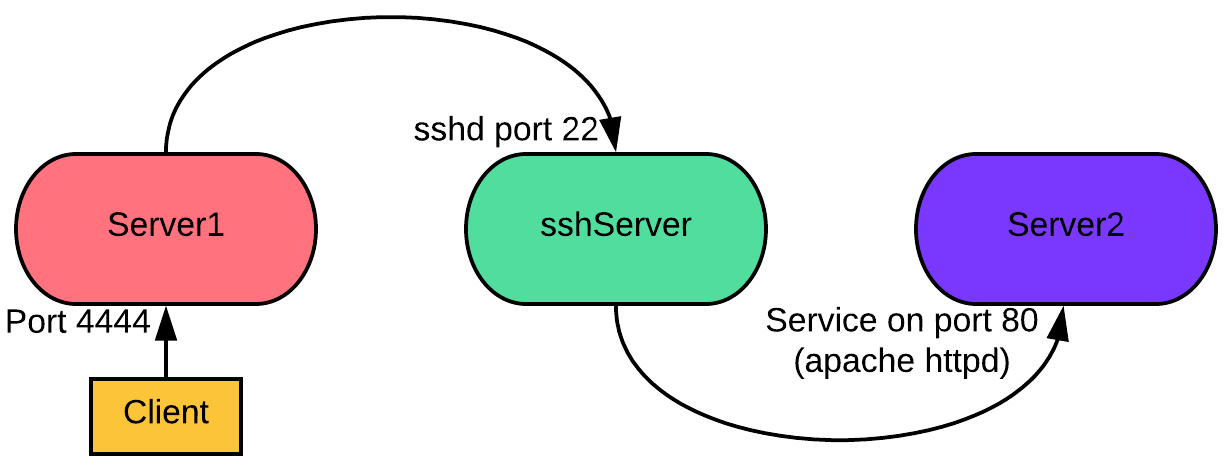
\includegraphics[width=0.9\linewidth]{Mod4/chapters/4.14.a}
	\caption{SSH Tunneling}
	\label{fig:4}
\end{figure}

	\section{Creating SSH Tunnels}
\subsection{Local port forwarding}
Let us consider in the previous example, that we want to forward \verb|duex.vm.somuvmnet.local|'s local port 4444 to \textit{port 80} on \verb|www.google.com|, through an SSH connection with the sshd process on \verb|prime.vm.somuvmnet.local|. In that case, we have to use the ssh command with the options \verb|-fNL|. The options stand for:

\noindent
\begin{tabular}{rM{0.85}}
	\toprule
	\textbf{Terms} &\textbf{Description} \\
	\midrule
	\textbf{-f}	&Turns the SSH session into a background process. The process can still ask for passwords, etc, but just before command execution it transitions to a background process.\\
	\midrule
	\textbf{-N}	&Do not execute remote commands - useful in this case to declare that this connection is specifically for \textit{port forwarding} and \textit{ssh tunneling}.\\
	\midrule
	\textbf{-L}	&Defines a local port on this host that should be forwarded to a remote port on another host.\\
	\bottomrule
\end{tabular}

\noindent
Thus, we start off by creating the ssh tunnel with:

\vspace{-15pt}
\begin{minted}{console}
# ssh -fNL 4444:www.google.com:80 root@prime.vm.somuvmnet.local 
Enter passphrase for key '/root/.ssh/id_ecdsa': 
#
\end{minted}
\vspace{-10pt}	

\noindent
The above command instructs the local port 4444 to be forwarded to Google.com's port 80, i.e., the webserver serving requests for google.com. This is to be done via an SSH tunnel created by the \textit{sshd} process on \verb|prime.vm.somuvmnet.local|. Thus, all requests to this server's \textit{port 4444} will automatically be sent to Google.com's port 80 via an encrypted SSH connection. Now, opening \verb|localhost:4444| on \verb|deux.vm.somuvmnet.local| will open google's homepage. 

We could also use a tunnel created by \textit{sshServer} (i.e., \verb|prime.vm.somuvmnet.local|) to visit a web page hosted by the \verb|httpd| process on sshServer itself, using:

\vspace{-15pt}
\begin{minted}{console}
# ssh -fNL 4444:localhost:80 root@prime.vm.somuvmnet.local
\end{minted}
\vspace{-10pt}	

\subsection{Remote port forwarding}
While less common, remote port forwarding is useful to connect a local port that is inaccessible from the internet (perhaps due to a firewall) to a remote port that is available to the internet. For example, if we want \verb|prime.vm.somuvmnet.local|'s \textit{port 8080} to be forwarded to \verb|deux.vm.somuvmnet.local|'s \textit{port 80}, i.e., when people go to \textit{port 8080} on the former, the web server on the latter serves, the requests, on \verb|deux.vm.somuvmnet.local| we have to type:

\vspace{-15pt}
\begin{minted}{console}
# ssh -R 80:localhost:8080 root@prime.vm.somuvmnet.local
\end{minted}
\vspace{-10pt}	

\noindent
The above would forward all data from the localhost on \verb|prime.vm.somuvmnet.local| to our local port 80. 

\subsection{Checking currently open SSH tunnels}
We can find out which ports are currently listening for incoming connections to forward, by filtering the list of open files, given by the \verb|lsof| command:

\vspace{-15pt}
\begin{minted}{console}
# lsof -i -n | grep ssh
sshd      1265   root    3u  IPv4  24321      0t0  TCP *:ssh (LISTEN)
sshd      1265   root    4u  IPv6  24336      0t0  TCP *:ssh (LISTEN)
ssh       4194   root    3u  IPv4  46794      0t0  TCP 10.0.99.12:35514->10.0.99.11:ssh (ESTABLISHED)
\end{minted}
\vspace{-10pt}	

\noindent
The \verb|-i| flag filters the output to internet related stuff. The \verb|-n| option prevents the reverse lookup of host IP addresses to FQDNs, to make the process faster. Without the flag, the output would be:

\vspace{-15pt}
\begin{minted}{console}
# lsof -i | grep ssh
sshd      1265   root    3u  IPv4  24321      0t0  TCP *:ssh (LISTEN)
sshd      1265   root    4u  IPv6  24336      0t0  TCP *:ssh (LISTEN)
ssh       4194   root    3u  IPv4  46794      0t0  TCP deux.vm.somuvmnet.local:35514->prime.vm.somuvmnet.local:ssh (ESTABLISHED)
\end{minted}
\vspace{-10pt}	

\noindent
Another useful tool for this purpose is \verb|netstat -tulpen|, which shows:

\vspace{-15pt}
\begin{minted}{console}
# netstat -tulpn | grep ssh
tcp        0      0 0.0.0.0:22              0.0.0.0:*               LISTEN      1265/sshd           
tcp        0      0 127.0.0.1:4444          0.0.0.0:*               LISTEN      4194/ssh            
tcp6       0      0 :::22                   :::*                    LISTEN      1265/sshd           
tcp6       0      0 ::1:4444                :::*                    LISTEN      4194/ssh      
\end{minted}
\vspace{-10pt}	